% !TEX TS-program = xelatex

% Copyright 2010 by Pedro Furlanetto 
%
% In principle, this file can be redistributed and/or modified under
% the terms of the GNU Public License, version 2.

% Based on Till Tantau beamer template

\documentclass{beamer}
%\documentclass[draft]{beamer}

\mode<presentation>
{
  \usetheme{Warsaw}
  \setbeamercovered{transparent}
}


\usepackage{hyperref}
\usepackage{graphicx}
\usepackage[english]{babel}
%\usepackage[utf8]{inputenc}
\usepackage{times}
\usepackage[T1]{fontenc}
\usepackage{xltxtra} % Extra customizations for XeLaTeX
\usepackage{color}
\usepackage{listings}
 

% "define" Scala
\lstdefinelanguage{Scala}{
  morekeywords={abstract,case,catch,class,def,%
    do,else,extends,false,final,finally,%
    for,if,implicit,import,match,mixin,%
    new,null,object,override,package,%
    private,protected,requires,return,sealed,%
    super,this,throw,trait,true,try,%
    type,val,var,while,with,yield}, % scala>
  otherkeywords={=,:,=>,<-,<\%,<:,>:,\#,@},
  sensitive=true,
  morecomment=[l]{//},
  morecomment=[n]{/*}{*/},
  morestring=[b]",
  morestring=[b]',
  morestring=[b]""",
 % literate={=>}{$\Rightarrow$ }2 {<-}{$\leftarrow$}2 {->}{$\rightarrow$}2
}


\definecolor{dkgreen}{rgb}{0,0.6,0}
\definecolor{gray}{rgb}{0.5,0.5,0.5}
\definecolor{mauve}{rgb}{0.58,0,0.82}

% Default settings for code listings
\lstset{frame=tb,
  language=Scala,
  aboveskip=3mm,
  belowskip=3mm,
  showstringspaces=false,
  columns=flexible,
  basicstyle={\scriptsize\ttfamily},
  numbers=none,
  numberstyle=\tiny\color{gray},
  keywordstyle=\color{blue},
  commentstyle=\color{dkgreen},
  stringstyle=\color{mauve},
  frame=single,
  breaklines=true,
  breakatwhitespace=true,
  tabsize=3,
  mathescape=true,
  resetmargins=true,
  showtabs=true
}

\setbeamertemplate{navigation symbols}{}%remove navigation symbols

\title{Scala Relâmpago}

%\subtitle{ \includegraphics[height=1cm]{lighting2.jpg}}

\author{Pedro Furlanetto}

\institute
{
  %Ideais Tecnologia\\
\begin{minipage}{0.6\textwidth}
\begin{flushleft} 

\includegraphics[height=1.5cm]{ideaisconf.png} 
\end{flushleft}
\end{minipage}
\begin{minipage}{0.3\textwidth}
\centering{ 
\includegraphics[height=2cm]{ideais-grande.jpg}}
\end{minipage}
  
}

\date[IC 2010] % (optional, should be abbreviation of conference name)
{IdeaisConf, 2010}

\subject{Linguagem de Programação Scala}

%\logo{
\includegraphics[height=1cm]{ideais-grande.jpg}}

\AtBeginSubsection[]
{
  \begin{frame}<beamer>{Resumo}
    \tableofcontents[currentsection,currentsubsection,sectionstyle=show/shaded,subsectionstyle=show/shaded/shaded]
  \end{frame}
}

%\beamerdefaultoverlayspecification{<+->}

\begin{document}

\begin{frame}  
 	\centering{
\includegraphics[height=1cm]{Scala_Logo2008.png}}
	\titlepage
\end{frame}

%\begin{frame}{Resumo}
%  \tableofcontents
%\end{frame}

\section{Overview}

\subsection{De onde veio e o que é Scala?}

\begin{frame}{Criada por} 
	\begin{itemize}
	\item Martin Odersky - \emph{École Polytechnique Fédérale de Lausanne} (EPFL), Lausanne, Switzerland em 2001
	\begin{itemize}
	   \item Ph.D. com \emph{Niklaus Wirth} (criador do Pascal)
              \item \emph{GJ} e \emph{Pizza} com \emph{Philip Wadler} - deu origem ao \emph{generics} do Java atual
	\end{itemize}	
	\end{itemize}
           \begin{columns}
           \begin{column}{.5\textwidth}
               \centering{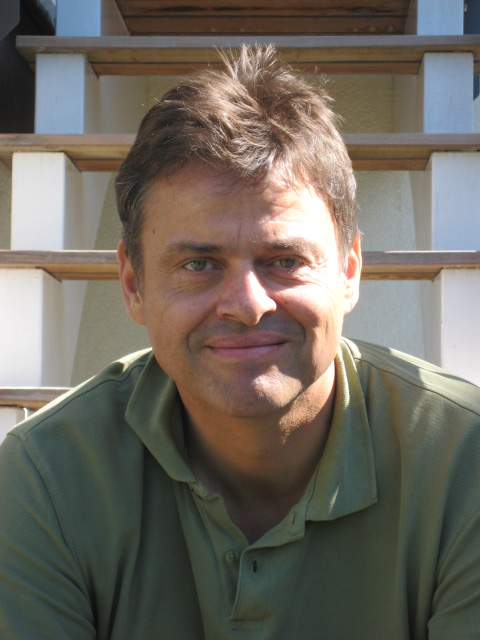
\includegraphics[height=4cm]{Martin-Odersky.jpg}}
           \end{column}
           \begin{column}{.5\textwidth}
               \centering{
\includegraphics[height=4cm]{scala-the-real-thing.jpg}}
           \end{column}
	\end{columns}
\end{frame}

\begin{frame}{Unifica funcional e orientação a objeto} 
    \centering{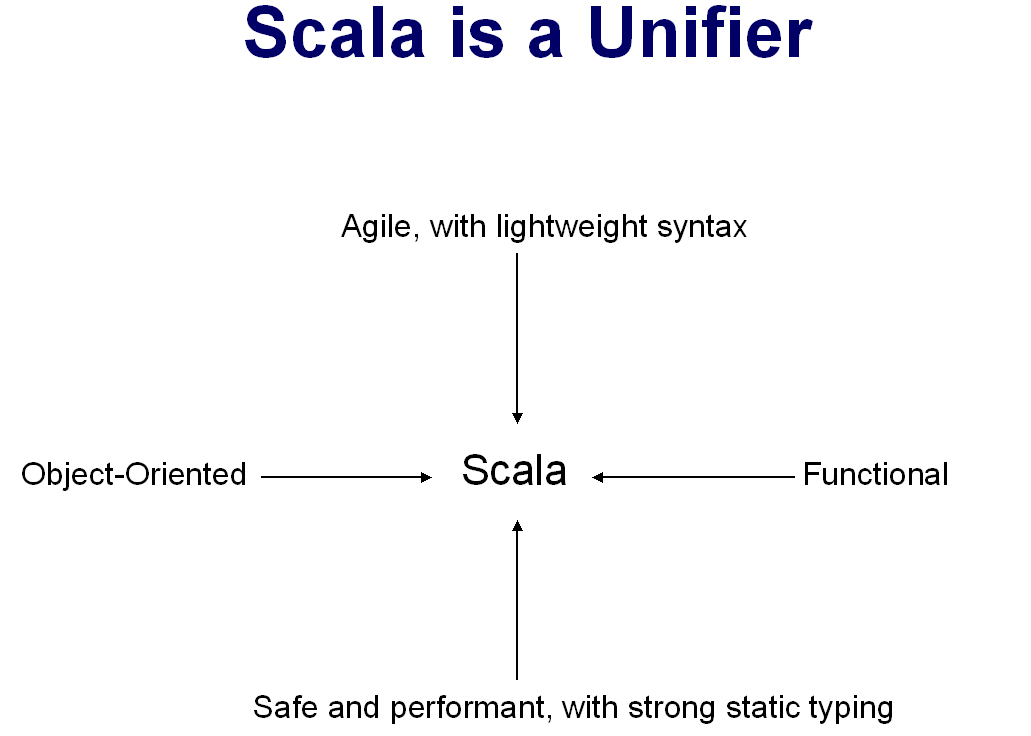
\includegraphics[scale=0.20]{Scala-is-a-Unifier.png}} 
\end{frame}

\begin{frame}[fragile]{Algumas características} 
    \begin{itemize} [<+->]
        \item Sintaxe simples e consistente 
        \begin{itemize}[<1->]
              \item Por exemplo: imports em qualquer lugar limitados pelo escopo, e imports
 de objetos
 	   \item Inferência de \textbf{;} 
        \end{itemize}
        \item Inferência de tipos 
        \item Baseado em expressões
        \begin{itemize}[<3->]
              \item tudo retorna alguma coisa - não precisa de \emph{return}
        \end{itemize}
        \begin{lstlisting}
	scala> val x:java.lang.Double = { import java.lang.Math._
	   max(1.71,1.72) 
	}
	x: java.lang.Double = 1.72	
	scala> val y = { import x._
	   intValue 
	}
	y: Int = 1
	\end{lstlisting}
       
    \end{itemize}
\end{frame}

\subsection{O básico}

\begin{frame}[fragile]{Algumas características} 
    \begin{itemize} [<+->]
        \item Tudo são objetos e chamadas de métodos (ala \emph{Smalltalk})
	\begin{lstlisting}
		                         1 + 5 * 4 == 1.+(5.*(4))
	 \end{lstlisting}
        \item Closures e funções como \emph{first-class citizens}
	\begin{lstlisting}
	scala> val string2int = (s:String) => Integer.parseInt(s)	
	string2int: (String) => Int = <function1>
	scala> string2int("5")
	Int = 5
	scala> List("g","j","z","a","r").sortWith { (x,y) => x < y }
	List[java.lang.String] = List(a, g, j, r, z)
	\end{lstlisting}
         \item Herança múltipla com \emph{traits e mixins}
    \end{itemize}
\end{frame}

\begin{frame}[fragile]{Algumas características} 
    \begin{itemize} %[<+->]
        \item Tuplas
        \item Accessors e Mutators automáticos - não presica ficar escrevendo \emph{getter} e  \emph{setter}
        \item Construtor e propriedades juntos
        \item Argumentos defaults e nomeados
		\begin{lstlisting}
		> class Exemplo(var nome:String = "<Sem Nome>", var idade:Int = 18)
		> val e = new Exemplo()
		> (e.idade, e.nome)
		$\textbf{(Int, String) = (18,<Sem Nome>)}$
		> val e2= new Exemplo(idade = 20)
		> (e2.idade, e2.nome)
		$\textbf{(Int, String) = (20,<Sem Nome>)}$
		\end{lstlisting}
    \end{itemize}
\end{frame}

\subsection{Um pouco alem do básico}

\begin{frame}[fragile]{Algumas características} 
    \begin{itemize} [<+->]
        \item Scala não tem \emph{métodos estáticos} - mas tem \emph{objetos companheiros}
        \begin{itemize}[<1->]
	\item Uma declaração \emph{object} no mesmo fonte e com o mesmo nome da classe
        \end{itemize}
        \item \emph{Case Classes}
        \begin{itemize}[<2->]
              \item Uma classe que já implementa \emph{hashCode}, \emph{equals}, \emph{clone} e \emph{toString} 
	   \item Também implementa um \emph{objeto companheiro} com os métodos \emph{apply} e \emph{unapply}
        \end{itemize}
        \item<3-> Método \emph{apply} funciona como um ``método default''
        \item<3-> Método \emph{unpply} serve para ``desconstruir'' uma classe
    \end{itemize}
\end{frame}

\begin{frame}[fragile]{Case Classes} 
    \begin{itemize} [<+->]
        \item Refazendo o exemplo como \emph{Case Classe} e um \emph{objeto companheiro}
	\begin{lstlisting}
	case class Exemplo(nome:String = "<Sem Nome>", idade:Int = 18)
	object Exemplo {
	  def media(e:Exemplo, e2:Exemplo) =
	     ( e.idade + e2.idade ) / 2
	}
	\end{lstlisting}
	\item Tuplas também podem ser usadas em atribuições
	\begin{lstlisting}
	> val (e,e2) = ( Exemplo(idade=20, nome="Fulano"), Exemplo("João",30) )
	e: Exemplo = Exemplo(Fulano,20)
	e2: Exemplo = Exemplo(João,30)
	> Exemplo.media(e,e2)
	Int = $\textbf{25}$
	\end{lstlisting}
    \end{itemize}
\end{frame}

\begin{frame}[fragile]{Andar, filtrar e colher dados de listas com facilidade} 
    \begin{itemize} %[<+->]
    \item<1-> Lembra do método \emph{apply} implementado pela \emph{case class} ? Ele é um \emph{factory method}.
    \item<1-> Usando \_ posso transformar métodos em funções
    
	\begin{lstlisting}
	> val E = Exemplo.apply _
	E: (String, Int) => Exemplo = <function2>
	
	> val lista = List(E("Roberto",34), E("Maria",15), E("João",18), E("Rosa",21), E("Fulana",8), E("Fulano",5), E("Ivo",30), E("Joana",10),E("Igor",18), E("Gustavo",21))
	\end{lstlisting}
	
	\item<2-> \emph{for-comprehensions} - todos os maiores de idade
	
	\begin{lstlisting}
	> val maiores = for(e <- lista; if e.idade >= 18 ) yield e
	maiores: List[Exemplo] = List(Exemplo(Roberto,34), Exemplo(João,18), Exemplo(Rosa,21), Exemplo(Ivo,30), Exemplo(Igor,18), Exemplo(Gustavo,21))	
	\end{lstlisting}
    \end{itemize}
\end{frame}

\begin{frame}[fragile]{Andar, filtrar e colher dados de listas com facilidade} 
    \begin{itemize} [<+->]
	\item Agora todos com a mesma idade, sem repetição
	\begin{lstlisting}
	> val mesmaIdade = for(
	      (e1, idx) <- lista.zipWithIndex; e2 <- lista.drop(idx + 1)
	      if e1 != e2 && e1.idade == e2.idade) 
	          yield  (e1, e2)
	mesmaIdade: List[(Exemplo, Exemplo)] = List((Exemplo(João,18),Exemplo(Igor,18)), (Exemplo(Rosa,21),Exemplo(Gustavo,21)))
	\end{lstlisting}

	\item \textbf{Calma!} Não é tão complicado.
	\begin{lstlisting}
	> lista.zipWithIndex.take(4)
	List[(Exemplo, Int)] = List((Exemplo(Roberto,34),0), (Exemplo(Maria,15),1), (Exemplo(João,18),2), (Exemplo(Rosa,21),3))
	\end{lstlisting}
    \end{itemize}
\end{frame}

\section{Um vislumbre... - Implicitos}

\subsection{Parâmetros}
\begin{frame}[fragile]{Implícitos} 
    \begin{itemize} [<+->]
	\item Voltando ao exemplo de ordenação
	\begin{lstlisting}
	          List("g","j","z","a","r").sortWith { (x,y) => x < y }
	\end{lstlisting}
	\item Poderiamos ter feito
	\begin{lstlisting}
	scala> List("g","j","z","a","r").sorted
	List[java.lang.String] = List(a, g, j, r, z)
	\end{lstlisting}
	\item<2-> Mas como ele sabe como ordenar?
	\item<3-> Veja a assinatura do método \emph{sorted}	
	\begin{lstlisting}
	def sorted (implicit ord: Ordering[A]) : List[A] 
	// $\emph{A}$ é o parâmetro genérico de List
	\end{lstlisting}
    \end{itemize}
\end{frame} 

\begin{frame}[fragile]{Implícitos} 
    \begin{itemize} [<+->]
	\item Existe um objeto implícito \emph{Ordering[String]} definido nas bibliotecas do Scala
	\begin{lstlisting}
	             implicit object String extends Ordering[String] 
	             // não conflita com String pois está em outro namespace
	\end{lstlisting}
	\item A nossa lista é do tipo \emph{List[String]}, portanto podemos rescrever a definição de List e a assinatura do método \emph{sorted} nesta forma ilustrativa 
	\begin{lstlisting}
	class List[String] {
	   def sorted(implicit ord: Ordering[String]) : List[String]
	}
	\end{lstlisting}
    \end{itemize}
\end{frame}

\begin{frame}[fragile]{Implícitos - como funciona?} 
    \begin{itemize} [<+->]
	\item Sempre que o compilador encontra um parâmetro implícito, um objeto implícito de tipo compatível é procurado, se encontrado é aplicado automaticamente. 
	\item Mas só quando um não é provido explicitamente.
	\begin{lstlisting}
	import scala.math.{Ordering=>Ord}	
	scala> List("g","j","z","a","r").sorted(Ord.String.reverse)
	List[java.lang.String] = List(z, r, j, g, a)
	\end{lstlisting}
	\item<2->  \emph{import scala.math.{Ordering=>Ord}} é um import normal mas fazendo um alias \emph{Ord} para \emph{Ordering}

    \end{itemize}
\end{frame}

\begin{frame}[fragile]{Implícitos} 
    \begin{itemize} [<+->]
	\item Vamos definir uma ordenação para o nosso exemplo
	\begin{lstlisting}
	class OrdemExemplo extends Ord[Exemplo] { 
	   def compare(x: Exemplo, y: Exemplo) = x.idade - y.idade 
	}
	implicit val ordemExemplo = new OrdemExemplo
	\end{lstlisting}
	\item Testando - e conferindo só os 5 primeiros 
	\begin{lstlisting}
	> lista.sorted.take(5)
	List[Exemplo] = List(Exemplo(Fulano,5), Exemplo(Fulana,8), Exemplo(Joana,10), Exemplo(Maria,15), Exemplo(João,18))
	\end{lstlisting}
	\item Sendo explicito
	\begin{lstlisting}	
	> lista.sorted(ordemExemplo.reverse).take(5)
	List[Exemplo] = List(Exemplo(Roberto,34), Exemplo(Ivo,30), Exemplo(Rosa,21), Exemplo(Gustavo,21), Exemplo(João,18))
	\end{lstlisting}
    \end{itemize}
\end{frame}

\subsection{Conversões}

\begin{frame}[fragile]{Implícitos - Conversões} 
    \begin{itemize} [<+->]
	\item Implícitos também são usados para converter dados de forma automática
	\item Vamos supor que tenhamos um CSV com nomes e idades
	\begin{lstlisting}
	> val csv="Crisão, 35\nFrancine, 25"
	
	> val listaArray = for(linha <- csv.lines.toList) yield linha.split(",")
	listaArray: List[Array[java.lang.String]] = 
	      List(Array(Crisão,  35), Array(Francine,  25))
	\end{lstlisting}
	\item Podemos construir um implícito que recebe \emph{Array[String]} e retorna \emph{Exemplo}
	\begin{lstlisting}
	> implicit def array2exemplo(arr: Array[String]):Exemplo =
	         Exemplo(arr(0), Integer.parseInt(arr(1).trim))
	> Exemplo.media(listaArray(0), listaArray(1))
	Int = 30
	\end{lstlisting}	
    \end{itemize}
\end{frame}

\subsection{\emph{Pimp-my-library}}

\begin{frame}[fragile]{Implícitos - \emph{Pimp-my-library}} 
    \begin{itemize} [<+->]
	\item Implícitos também podem ser usados para ``simular'' a introdução de métodos em classes já existentes.
	\item Poderiamos criar um método que transformasse um \emph{String} em \emph{Exemplo}
	\begin{lstlisting}
	> implicit def pimpedString(s:String) = new {
	     def toExemplo:Exemplo = s.split(",") 
	}
	\end{lstlisting}
	\item Repare que \emph{s.split} obviamente retorna \emph{Array[String]}, mas o nosso \emph{array2exemplo} se encarrega de converte-lo. Por isso \emph{toExemplo} tem seu retorno declarado explicitamente
	\begin{lstlisting}
	> "Zeca, 66".toExemplo
	Exemplo = Exemplo(Zeca,66)
	
	> for(linha <- csv.lines.toList) yield linha.toExemplo
	List[Exemplo] = List(Exemplo(Crisão,35), Exemplo(Francine,25))
	\end{lstlisting}	
    \end{itemize}
\end{frame}

\section{Conclusão}

\subsection{O que não vimos?}

\begin{frame}{O que não vimos?}
	\begin{itemize} %[<+->]
	\item \emph{Coleções} - \emph{map}, \emph{fold}, \emph{reduce}
	\item \emph{Traits} e \emph{Mixins} - Herança multipla controlada
	\item \emph{Pattern Matches}
	\item \emph{Self-types} - Representando dependencias entre classes e traits 
	\item \emph{Tipos estruturais} - a.k.a. \emph{Duck typing done right}
	\item \emph{Option objects} - null object
	\item \emph{Parâmetros por nome} - ``avaliação tardia''
	\item \emph{Type classes} 
	
	\vfill
	\centering{\textbf{E MUITO MAIS}}
	\end{itemize}
\end{frame}

\subsection{Será que é complicado?}

\begin{frame}[fragile]{Será que é complicado?}
   \begin{itemize}% [<+->]
	\item Sim, pode ser complicado
	\begin{lstlisting}
	trait MA[M[_], A] {
	  val value: M[A]
	  def convertTo[N[_]](implicit c: M #==> N): N[A] = c[A](value)
	}
	\end{lstlisting}
	\item Parte de um código que usa a biblioteca de parsing
	\begin{lstlisting}
	def trans: Parser[List[LineItem]] =  "(" ~> repsep(trans_spec, ",") <~ ")" ^^ { (ts: List[LineItem]) => ts }
	def trans_spec: Parser[LineItem] = buy_sell ~ buy_sell_instr ^^ { case bs ~ bsi => new LineItem(bsi._1._2, bsi._1._1, bs, bsi._2) }
	def account_spec =  "for" ~> "trading" ~> "account" ~> stringLit ^^ {case s => s}
	def buy_sell: Parser[ClientOrder.BuySell] =   ("buy" | "sell") ^^ { case "buy" => ClientOrder.BuySell.BUY;  case "sell" => ClientOrder.BuySell.SELL }
	\end{lstlisting}
\end{itemize}
\end{frame}

\begin{frame}[fragile]{Será que é complicado?}
%   \begin{itemize} [<+->]
	
	\centering{\textbf{Só se você quiser!}}
	\vfill
	\begin{columns}
           \begin{column}{.5\textwidth}               
              \centering{``\emph{Com grandes poderes vêm grandes responsabilidades.}''}
           \end{column}
           \begin{column}{.5\textwidth}
               
\includegraphics[height=5cm]{spiderman.png}
           \end{column}
	\end{columns}
	
%\end{itemize}
\end{frame}

\subsection{Referências}

\begin{frame}{Para aprender mais}
	\begin{itemize} 
	\item \url{http://www.scala-lang.org}
		\begin{itemize} 
			\item A Tour of Scala
			\item Scala by Example
			\item A Brief Scala Tutorial
		\end{itemize}
	\item \url{http://planetscala.org} - agregador de blogs sobre Scala
	\item \emph{Programming Scala} - Martin Odersky, Lex Spoon, and Bill Venners - Artima
	\item \emph{Programming Scala} - Dean Wampler, Alex Payne - O’Reilly Media 
	\begin{itemize} 
		\item Online: \url{http://programming-scala.labs.oreilly.com/}
	\end{itemize}

	\end{itemize}
\end{frame}

%\begin{frame}[fragile]{\emph{Pattern Matches}} 
%    \begin{itemize} %[<+->]
%	\item ``Descontruir'' objetos com facilidade
%	\begin{lstlisting}	
%	> lista(0)
%	Exemplo = Exemplo(Roberto,34)
%	
%	> val Exemplo(nome,idade) = lista(0)
%	nome: String = Roberto
%	idade: Int = 34
%	\end{lstlisting}
%	
%	\item Ou só uma parte do objeto
%	\begin{lstlisting}	
%	> lista.collect { case Exemplo(nome,18) => nome }
%	List[String] = List(João, Igor)	
%	\end{lstlisting}
%    \end{itemize}
%\end{frame}

\end{document}


